\documentclass{article}
\usepackage{amssymb}
\usepackage{mdwlist}
\usepackage{mathtools}
\usepackage{tikz}
\usepackage[utf8]{inputenc}
\usepackage[english]{babel}
\usepackage{amsthm}

\addtolength{\oddsidemargin}{-.875in}
\addtolength{\evensidemargin}{-.875in}
\addtolength{\textwidth}{1.75in}
\addtolength{\topmargin}{-.875in}
\addtolength{\textheight}{1.75in}


\newtheorem{theorem}{Theorem}
\renewcommand\qedsymbol{$\blacksquare$}

\begin{document}
	%\pagenumbering{gobble}
 	\noindent\Large{Math Notes: August 2011 - May 2020 \hfill Ian McDowell}
	\noindent\hrule

	\section*{Table of Contents}
	\begin{enumerate*}
		\item Math 7 for 6th Graders (Fall 2011-Spring 2012)\hfill Page 2
		\item Math 8 for 7th Graders (Fall 2012-Spring 2013)
		\item Algebra I (Fall 2013-Spring 2014)
		\item Honors Geometry (Fall 2014-Spring 2015)
		\item Algebra II (Fall 2015-Spring 2016)
		\item MAT 110: College Algebra (Fall 2016)
		\item MAT 111: College Trigonometry (Spring 2017)
		\item MAT 140: Analytic Geometry and Calculus I (Fall 2017)
		\item MAT 120: Probability and Statistics (Spring 2018)
		\item MATH 142: Calculus II (Fall 2018)
		\item MATH 241: Calculus III (Spring 2019)
		\item MATH 300: Transition to Advanced Mathematics (Spring 2019)
		\item MATH 544: Linear Algebra (Fall 2019)
		\item MATH 574: Discrete Mathematics I (Fall 2019)
		\item MATH 520: Ordinary Differential Equations (Spring 2020)
		\item MATH 532: Modern Geometry (Spring 2020)
		\item MATH 552: Applied Complex Variables (Spring 2020)
	\end{enumerate*}

	\newpage
\noindent\Large{Math 7 for 6th Graders (Fall 2011-Spring 2012)}
\noindent\hrule

	\section*{Math 7 for 6th Graders:}
	\begin{enumerate*}
		\item[\Large\textbf{1-1}] \Large\textbf{Intro to Algebra and Functions (The Plan for Problem Solving):}\\
			\begin{enumerate*}
				\item[$\bullet$] Understand\\
					What do you know?\\
					What do you want to know?\\
					Do you have too much or too little information?\\
				\item[$\bullet$] Plan\\
					How do the facts relate to each other?\\
					What is a reasonable strategy?\\
				\item[$\bullet$] Solve\\
					Use your plan and get an answer.\\
				\item[$\bullet$] Check\\
					Does your answer make sense?\\
					If not, try another approach!\\
			\end{enumerate*}
			
		\item[\Large\textbf{1-2}] \Large\textbf{Powers and Exponents:}\\
			\begin{enumerate*}
			\item[$\bullet$]\textbf{Factor} - A number used in a multiplication problem (Example: 2$\times$1)\\
			In $3^2$:\\ 3 is called the \textbf{base} and 2 is called the \textbf{exponent}.\\
			This means that 3 is used as a factor twice (the product is 9)\\ $3^2=3\times3=9$\\
			
\newpage
\noindent\Large{Math 7 for 6th Graders\hfill 1-2 Powers and Exponents}
\noindent\hrule
\vspace{5mm}

			\item[$\bullet$]\textbf{Power} - A number that can be written using an exponent.\\
			To the $2^{nd}$ power can also be called ``Squared''.\\
			To the $3^{rd}$ power can also be called ``Cubed''.\\
			To evaluate powers, you multiply the factors.\\
			A number is in standard form if it does not contain any exponents\\
			$2^3=2\times2\times2=8$\\
			\item[$\bullet$]Powers - $5^2;8^3;2^4$\\
			Squared - $5^2$\\
			Cubed - $8^3$\\
			Base - $5^2:5;8^3:8;2^4:2$\\
			Exponent - $5^2:2;8^3:3;2^4:4$\\
			Factors - $5^2:5\times5$; $8^3:8\times8\times8$; $2^4:2\times2\times2\times2$\\
			\end{enumerate*}
			
		\item[\Large\textbf{1-3}] \Large\textbf{Squares and Square Roots:}\\
			Numbers that are squares of whole numbers are called \textbf{perfect squares}.\\
			Square Roots:\\
			If $a^2=b$ then a is the square root of b.\\
			$2\times2=4$\\
			$\sqrt{b}=a$; $\sqrt{4}=2$\\
			This is called a radical sign: $\sqrt{}$\\
			Perfect Squares:\\
			$1^2 = 1; 2^2=4; 3^3=9; 4^2=16; 5^2=25; 6^2=36; 7^2=49; 8^2=64; 9^2=81;$\\
			$10^2=100; 11^2=121; 12^2=144; 13^2=169; 14^2 = 196; 15^2=225;$\\
			$16^2=256; 17^2=289; 18^2=324; 19^2=361; 20^2=400; 21^2=441$\\
			$22^2=484; 23^2=529; 24^2=576; 25^2=625; ...$\\
			If you know the area of a square, then the square root of the area will be the length of one of the sides of the square.\\
			
		\item[\Large\textbf{1-4}] \Large\textbf{Order of Operations:}\\
			PEMDAS - ``Please Excuse My Dear Aunt Sally''\\
			
\newpage
\noindent\Large{Math 7 for 6th Graders\hfill 1-4 Order of Operations}
\noindent\hrule
\vspace{5mm}
			
			\begin{enumerate*}
			\item[$\bullet$]P\\
				Parentheses/Grouping Symbols\\
				Also includes brackets [ ] and ``invisible'' parentheses in the numerator and denominator of a fraction.\\
				$\frac{8-2}{3}=\frac{(8-2)}{3}=\frac{6}{3}$\\
			\item[$\bullet$]E\\
				Exponents\\
				Note: $2+3^2$ is not the same as $(2+3)^2$\\
				$2+3^2=2+9=11$\\
				$(2+3)^2=5^2=25$\\
			\item[$\bullet$]M/D\\
				Multiply/Divide\\
				They are done IN ORDER from LEFT to RIGHT.\\
			\item[$\bullet$]A/S\\
				Addition/Subtraction\\
				Also done in order from left to right.\\
			\end{enumerate*}
			
		\item[\Large\textbf{1-6}] \Large\textbf{Variables and Expressions:}\\
			\begin{enumerate*}
				\item[$\bullet$]\textbf{Variable}: A symbol, usually a letter, that stands for a number in a mathematical expressions and sentences.\\
				\item[$\bullet$]\textbf{Algebra}: The branch of math using numbers and letters.\\
				\item[]An \textbf{Algebraic Expression} is an expression consisting of number(s), variable(s), and operation(s).\\
					To evaluate an expression, you must be told what numbers to substitute for the variables.\\
					Rewrite the problem with these values and solve using PEMDAS.
				\item[$\bullet$]Ways to write multiply:\\
					$a\cdot b$; $a\times b$; $a(b)$; $ab$; $3b$ (coefficient)\\
					
\newpage
\noindent\Large{Math 7 for 6th Graders\hfill 1-6 Variables and Expressions}
\noindent\hrule
\vspace{5mm}
			
			\item[$\bullet$]Ways to write divide:\\
				$a\div b$; $a\overline{)b}$; $\frac{a}{b}$\\
			\item[$\bullet$]Examples:\\
				$n=6, p=4$; $6n-p=32$; $n^2+5=41$\\
			 \item[$\bullet$]Evaluate each expression if $a=6 b=3 c=2$:\\
			 	1. $a-b+5=8$\\
			 	2. $c\times a\times b=36$\\
			 	3. $\frac{ca}{b}-c=2$\\
			 	4. $c(a+b)-c=16$\\			
			\end{enumerate*}
			
		\item[\Large\textbf{1-7}] \Large\textbf{Equations:}\\
			\begin{enumerate*}
				\item[$\bullet$]\textbf{Equation}: A mathematical sentence which contains an equals(=) sign.\\
				\item[$\bullet$]\textbf{Solution}: The number which makes the sentence true.\\
				\item[] The process of finding the solution is called \textbf{solving the equation}.\\
					Some equations can be solved using mental math.\\
			\end{enumerate*}
			
		\item[\Large\textbf{1-8}] \Large\textbf{Properties:}\\
			\begin{enumerate*}
				\item[$\bullet$]\textbf{Property}: Statement that is true for all numbers.\\
				\item[$\bullet$]\textbf{Commutativity}: The order of numbers does not matter.\\
					\item[]\textbf{Commutative Property of Addition}:\\
						$a+b=b+a$; $9001+70=70+9001$\\
					\item[]\textbf{Commutative Property of Multiplication}:\\
						$a\times b=b\times a$; $(70)(9001)=(9001)(70)$\\
					
\newpage
\noindent\Large{Math 7 for 6th Graders\hfill 1-8 Properties}
\noindent\hrule
\vspace{5mm}
					
				\item[$\bullet$]\textbf{Associativity}: The order of the same operation does not matter.\\
					\item[]\textbf{Associative Property of Addition}:\\
						$a+(b+c)=(a+b)+c$; $1+(2+3)=(1+2)+3$\\
					\item[]\textbf{Associative Property of Multiplication}:\\
						$a(bc)=(ab)c$; $1\times(2\times3)=(1\times2)\times3$\\
				\item[$\bullet$]\textbf{Identity Property of Addition}:\\
					$a+0=a$; $20+0=20$\\
				\item[$\bullet$]\textbf{Identity Property of Multiplication}:\\
					$1\times a=a$; $1\times20=20$\\
				\item[$\bullet$]\textbf{Distributive Property}:\\
					$a(b+c)=ab+ac$; $2(3+6)=2(3)+2(6)=6+12=18$\\
			\end{enumerate*}

		\item[\Large\textbf{1-9}] \Large\textbf{Sequences:}\\
			\begin{enumerate*}
				\item[$\bullet$]\textbf{Sequence}: List of numbers in a specific order.\\
				\item[]Each number in a sequence is called a \textbf{term}.\\
				\item[]If you are adding/subtracting the same number each time, it is called an \textbf{Arithmetic Sequence}.\\
				\item[]If you are multiplying/dividing by the same number each time, it is called a \textbf{Geometric Sequence}.\\
				\item[]If there is a pattern but it is neither of the above, we will refer to the sequence as ``neither''.\\
			\end{enumerate*}

\newpage
\noindent\Large{Math 7 for 6th Graders\hfill 1-10 Equations and Functions}
\noindent\hrule
\vspace{5mm}

		\item[\Large\textbf{1-10}] \Large\textbf{Equations and Functions:}\\
			\begin{enumerate*}
				\item[]A relationship that has exactly one output value for each input value is called a \textbf{function}.\\
					The operation to be performed on the input is contained in the \textbf{function rule}.\\
				\item[]The set of input values is called the \textbf{domain}.\\
				\item[]The set of output values is called the \textbf{range}.\\
					The domain, range, and rule can be organized in a function table\\
				\item[]Functions are often written as equations with 2 variables where x is the input and y is the output.\\
			\end{enumerate*}
			
		\item[\Large\textbf{1-11}] \Large\textbf{Scientific Notation:}\\
			Powers of 10:\\
			$10^1=10; 10^2=100; 10^3=1,000; ...; 10^8=100,000,000$\\
			$10^{-1}=0.1; 10^{-2}=0.01; 10^{-3}=0.001; ...; 10^{-6}-0.000001$\\
			\textbf{Standard Form}:\\
				$785,000,000.; 0.0000075; 38,600$\\
			\textbf{Scientific Notation}:\\
				$7.85\times10^8; 7.5\times10^{-6}; 3.86\times10^4$\\
				
		\item[\Large\textbf{2-1}] \Large\textbf{Integers:}\\
			\begin{enumerate*}
				\item[]If temperatures fall below freezing, how do we write them using the celsius scale?\\
				\item[$\bullet$]Numbers greater than 0 are called \textbf{positive}.\\
				\item[$\bullet$]Numbers less than 0 are called \textbf{negative}.
				\item[$\bullet$]\textbf{Integers}:\\
				\item[]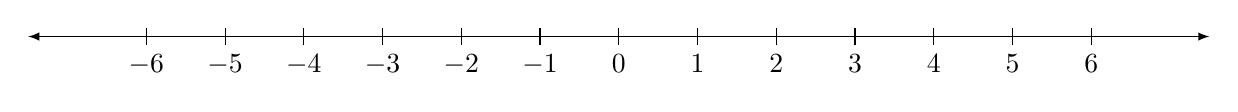
\begin{tikzpicture}[scale=1]
					\draw[latex-latex] (-7.5,0) -- (7.5,0) ;
					\foreach \x in  {-6,-5,-4,-3,-2,-1,0,1,2,3,4,5,6}
					\draw[shift={(\x,0)},color=black] (0pt,3pt) -- (0pt,-3pt);
					\foreach \x in {-6,-5,-4,-3,-2,-1,0,1,2,3,4,5,6}
					\draw[shift={(\x,0)},color=black] (0pt,0pt) -- (0pt,-3pt) node[below] 
					{$\x$};
				\end{tikzpicture}
					
\newpage
\noindent\Large{Math 7 for 6th Graders\hfill 2-1 Integers}
\noindent\hrule
\vspace{5mm}
					
				\item[$\bullet$]\textbf{Absolute Value}: A number's distance from zero on a number line. The distance is always positive and the absolute value of x looks like $|x|$.\\
					What is the relationship between an integer and its absolute value?\\
			\end{enumerate*}
			
		\item[\Large\textbf{2-2}] \Large\textbf{Comparing and Ordering Integers:}\\
			\begin{enumerate*}
				\item[]It is wise to imagine an integer's location on a number line.\\
				Positive numbers are always greater than negative numbers and negative numbers are always smaller than positive numbers.\\
				0 is smaller than all positive numbers and larger than all negative numbers.\\
				Be careful with negative numbers. The smaller its absolute value, the larger it is and the larger its absolute value, the smaller it is.\\
				Example: $|-4|=4; |31-30|=|1|=1$\\
				\item[$\bullet$]Operators:
					$<$ less than\\ $>$ greater than\\ $\leq$ less than or equal to\\ $\geq$ greater than or equal\\ $=$ equal to\\
			\end{enumerate*}
			
		\item[\Large\textbf{2-3}] \Large\textbf{Addition of Integers:}\\
			\begin{enumerate*}
				\item[$\bullet$]\textbf{Additive Inverse/Opposite}: A number added to its additive inverse equals zero.\\
				$7+-7=0$
				\item[]When you subtract integers you first have to rewrite the subtraction problem as an addition problem. How do you do this?\\
				You change the $-$ sign to a $+$ and add the opposite of the $2^{nd}$ number, then you apply the rules of addition.\\
				Example: $10-4=10+(-4)=6$\\
			\end{enumerate*}
			
\newpage
\noindent\Large{Math 7 for 6th Graders\hfill 2-4 Subtraction of Integers}
\noindent\hrule
\vspace{5mm}
			
		\item[\Large\textbf{2-4}] \Large\textbf{Subtraction of Integers:}\\
			Subtracting integers is the opposite of adding. You change the $+$ sign to a $-$ sign and subtract the opposite of the $2^{nd}$ number.\\
			Example: $15+(-20)=15-20=-5$\\
			
		\item[\Large\textbf{2-5}] \Large\textbf{Multiplication and Division of Integers:}\\
			When multiplying and dividing integers, first count the amount of negative signs.\\
			If there is an odd number of negative signs, the answer is negative. If there is an even number of negative signs, the answer is positive.\\
			Example: $-7(-13)=91; -27\div9=-3$\\
			
		\item[\Large\textbf{3-1}] \Large\textbf{Linear Equations and Functions:}\\
			In word problems, translate from english to math.
			\begin{enumerate*}
			 \item[$\bullet$]An expression has no $=$ sign.
			 \item[$\bullet$]Define the variables in the problem.
			 \item[$\bullet$]Translate the problem into an equation.\\
			 Multiplication words: Of\\
			 Division words: Per, Into\\
			 Halve: $\frac{1}{2}=\div2$\\
			 Examples: Nine less 2 is 7 = $9-2=7$\\
			 \end{enumerate*}
			 
		\item[\Large\textbf{3-2}] \Large\textbf{Solving Equations by Addition and Subtraction:}\\
			The goal of solving equations is to isolate the variable on one side of the $=$ sign. We do this by performing \textbf{inverse operations}.\\
			$-2+y=10$ Add 2 to both sides.\\$-2+y+2=10+2$\\$y=12$\\
			\textbf{Addition Property of Equality}: If $a=b$ then $a+c=b+c$\\
			\textbf{Subtraction Property of Equality}: If $a=b$ then $a-c=b-c$\\
		
\newpage
\noindent\Large{Math 7 for 6th Graders\hfill 3-3 Solving Equations by Mult. and Div.}
\noindent\hrule
\vspace{5mm}
				
		\item[\Large\textbf{3-3}] \Large\textbf{Solving Equations by Multiplication and Division:}\\
			\textbf{Multiplication Property of Equality}: If $a=b$ then $ac=bc$\\
			\textbf{Division Property of Equality}: If $a=b$ then $\frac{a}{c}=\frac{b}{c}$ if $c\neq0$\\
			$\frac{x}{2}=5$ Multiply both sides by 2\\$\frac{x}{2}\cdot2=5\cdot2$\\$x=10$\\
			
		\item[\Large\textbf{3-4}] \Large\textbf{Solving Two-Step Equations:}\\
			The order changes from PEMDAS to SADMEP. You add and subtract first then multiply and divide.\\
			$3y+10-7=6$\hfill$-2y-7.2=18.2$; Add 7.2 \\
			$3y+3=6$; Subtract 3 \hfill$-2y=25.4$; Divide by -2\\
			$3y=3$; Divide by 3\hfill$y=12.7$\\$y=1$\\
			
		\item[\Large\textbf{4-5}] \Large\textbf{Inequalities:}\\
			$<$ Less than:\hfill
			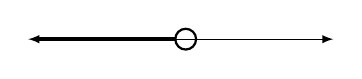
\begin{tikzpicture}[scale=2.5]
				\draw[very thick] (-3.5,0) -- (-2.75,0);
				\path [draw=black, fill=white, thick] (-2.75,0.0) circle (1.5pt);
				\draw[latex-latex] (-3.55,0) -- (-2,0) ;
			\end{tikzpicture}\\
			$>$ Greater than:\hfill
			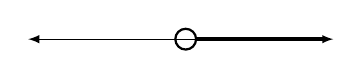
\begin{tikzpicture}[scale=2.5]
				\draw[very thick] (-2.75,0) -- (-2.05,0);
				\path [draw=black, fill=white, thick] (-2.75,0.0) circle (1.5pt);
				\draw[latex-latex] (-3.55,0) -- (-2,0) ;
			\end{tikzpicture}\\
			$\leq$ Less than or equal to:\hfill
			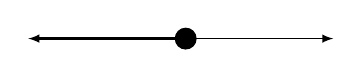
\begin{tikzpicture}[scale=2.5]
				\draw[very thick] (-3.5,0) -- (-2.75,0);
				\path [draw=black, fill=black] (-2.75,0.0) circle (1.5pt);
				\draw[latex-latex] (-3.55,0) -- (-2,0) ;
			\end{tikzpicture}\\
			$\geq$ Greater than or equal to:\hfill
			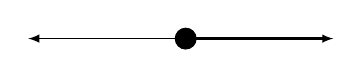
\begin{tikzpicture}[scale=2.5]
				\draw[very thick] (-2.75,0) -- (-2.05,0);
				\path [draw=black, fill=black] (-2.75,0.0) circle (1.5pt);
				\draw[latex-latex] (-3.55,0) -- (-2,0) ;
			\end{tikzpicture}\\
			$\neq$ Unequal to\\
			Inequalities are solved the same way as equations.\\
			$y-7=5$; Add 7\hfill$y-7<5$; Add 7\\
			$y=12$\hfill$y<12$\\
			When multiplying or dividing by positive numbers, the statement continues to be true, but when multiplying or dividing by negative numbers, you need to reverse the inequality symbol for the inequality to still be true.\\
			
		\item[\Large\textbf{4-6}] \Large\textbf{Fractions and Decimals:}\\
		\item[\Large\textbf{4-7}] \Large\textbf{Fractions and Percents:}\\
		\item[\Large\textbf{4-8}] \Large\textbf{Comparing and Ordering Rational Numbers:}\\
		\item[\Large\textbf{5-2}] \Large\textbf{Adding and Subtracting Fractions:}\\
		\item[\Large\textbf{5-3}] \Large\textbf{Multiplying and Dividing Fractions and Mixed Numbers:}\\
		\item[\Large\textbf{5-6}] \Large\textbf{Solving Equations:}\\
		\item[\Large\textbf{6-1}] \Large\textbf{Ratios and Proportions:}\\
		\item[\Large\textbf{6-2}] \Large\textbf{Rates:}\\
		\item[\Large\textbf{6-3}] \Large\textbf{Rates of Change:}\\
		\item[\Large\textbf{6-6}] \Large\textbf{Solving Proportions and Direct vs. Indirect Proportions:}\\
		\item[\Large\textbf{6-8}] \Large\textbf{Scale Drawings:}\\
		\item[\Large\textbf{Misc-1}] \Large\textbf{Customary Units:}\\
		\item[\Large\textbf{Misc-2}] \Large\textbf{Converting Between Systems:}\\
		\item[\Large\textbf{Misc-3}] \Large\textbf{The Percent Proportion:}\\
		\item[\Large\textbf{7-6}] \Large\textbf{Percent of Change:}\\
		\item[\Large\textbf{7-7}] \Large\textbf{Sales Tax, Discount, and Simple Interest:}\\
		\item[\Large\textbf{8}] \Large\textbf{Measures of Central Tendency and Range:}\\
		\item[\Large\textbf{9-7}] \Large\textbf{Theoretical and Experimental Probability:}\\
		\item[\Large\textbf{9-8}] \Large\textbf{Compound Events:}\\
		\item[\Large\textbf{10-3}] \Large\textbf{Circle Graphs:}\\

	\end{enumerate*}

\end{document}